\documentclass[11pt]{iopart}
\usepackage[utf8]{inputenc}
\usepackage[T1]{fontenc}
\usepackage{gensymb}

\usepackage[left]{lineno}
\linenumbers

\usepackage{setspace}
\doublespacing

\usepackage[
maxbibnames=99,
maxcitenames=2,
uniquelist=false,
uniquename=false,
backend=biber,
style=authoryear,
doi=false,isbn=false,url=false
]{biblatex}
\addbibresource{references.bib}
\AtEveryBibitem{%
  \clearlist{language}%
}

% Keywords command
\providecommand{\keywords}[1]
{
  \small	
  \textbf{\textit{Keywords---}} #1
}

\usepackage{mathtools}

%\DeclarePairedDelimiterX{\infdivx}[2]{(}{)}{%
%  #1\;\delimsize\|\;#2%
%}
%\newcommand{\infdiv}{D\infdivx}
%\DeclarePairedDelimiter{\norm}{\lVert}{\rVert}


\begin{document}

\title{Hydroclimate variability influenced social interaction in the prehistoric American Southwest}

\author{Nicolas Gauthier$^1$}

\address{$^1$ School of Human Evolution and Social Change, 900 S Cady Mall, Tempe, USA}

\ead{Nicolas.Gauthier@asu.edu}

\begin{abstract}
  In agricultural societies, farmers use their social networks to absorb the impacts of droughts and floods by facilitating resource flows to affected settlements and population flows away from them. These benefits depend on the degree to which a social network connects populations in topographically accessible locations that tend to experience different weather patterns. Here I use an empirical archaeological case study from the late pre-Hispanic period in the North American Southwest to examine the relationship between drought variability and human social networks. I analyze 7.5 million artifacts collected from nearly 500 archaeological sites, and estimate how the flow of social information between sites varied as a function of distance and growing-season hydroclimate variability over a period of 250 years. I find that although the intensity of social interaction was highly distance dependent, interaction between regions experiencing different oceanic and continental air masses is higher than would be expected by chance and distance alone. This work highlights the importance of distinguishing between different dynamic origins of drought variability when considering the social impacts of droughts and pluvials in the past and present.
\end{abstract}

\noindent{\it Keywords\/}: drought patterns, archaeological networks, spatial interaction model 

\maketitle

%\ioptwocol

\section*{Introduction}

Exchange networks are part of the broad toolkit of social and physical infrastructure human populations use to manage environmental risk in social-ecological systems \parencite{Anderies2015}. The biophysical environment can structure many of the costs and benefits of social interaction, as it does with physical infrastructure. Recent theoretical and empirical work highlights how spatial, social, and environmental factors influence networks of exchange and interaction \parencite{Fafchamps2007,Bloch2008,Nolin2010,Verdery2012,Freeman2014,Koster2014,Hao2015a,Schnegg2015}. Distance often emerges as an important factor in such systems. For agricultural societies in water-limited environments, hydroclimate variability -- specifically the balance of precipitation and evapotranspiration -- is another critical factor. The benefits of interacting with others in distinct drought regimes will often outweigh the costs of traveling longer distances. As a consequence, we might expect a greater ``investment of social energy in the maintenance of social ties'' between populations experiencing poorly or negatively correlated climate variability \parencite{Rautman1993a}. Norms and institutions that maintain ties between different climate regimes are likely to evolve \parencite{Durante2009}. This process is difficult to measure in the present day due to the mismatch between the generational time scale on which cultural evolution occurs and the limited time horizons available to contemporary social sciences. We can instead turn to the archaeological record for answers. 

Archaeology focuses on the material correlates of human behavior and is unique in addressing how social and physical infrastructure modulates human interactions with the environment over long time spans. Not only do archaeologists catalogue the remains of field systems, road networks, canals, and other components of hard infrastructure directly, but also the ceramics, raw materials, and luxury goods that are the material correlates of past networks of exchange and interaction. A powerful idea in archaeology is that, because of the interactions between societies and their biophysical environments, the spatial and temporal patterns of environmental variability can be used to predict ``ideal'' cultural responses and compared to archaeological observations \parencite{Halstead1989}. Yet in practice it is often difficult to find archaeological data fit for purpose, due to the incomplete nature of the archaeological record and the paucity of detailed paleoclimate data at the scales most relevant to human populations. 
%The need to address this issue extends beyond archaeological interest, and its importance is not limited to the past. over 90\% of the world's small farms are , and these farmers rely on complex networks of formal and informal arrangements in much the same way as their forbears have for 1,000s of years. Tracing the flows of information and energy within these complex social-ecological systems is essential for understanding their long-term behavior, and leveraging our archaeological understanding of why societies succeed or fail will be critical to anticipating the impact of impending climate changes on farming communities in the developing world.

The North American Southwest, however, is an exception. The climate of this region has been intensively studied by paleoclimatologists and climate modelers \parencite{Cook1999,Sheppard2002,McCabe2004,Herweijer2007a, Cook2011,Bocinsky2014, Coats2015a, Ault2018}. Additionally, nearly two centuries of survey and excavation have yielded extensive, high quality settlement pattern data \parencite{Hill2004}. Rates of archaeological site preservation and recovery in the Southwest are exceptionally high due to the arid climate, and comparatively low density of Euro-American occupation. Hence, detailed inventories of material culture at hundreds of archaeological sites provide an unparalleled view of the structure and dynamics of past social networks. This archaeological record attests to extensive exchange networks of durable goods such as ceramics and obsidian \parencite{Malville2001,Taliaferro2010,Mills2013a}, and there is direct (if limited) evidence for the long-distance transport of limited quantities of maize to the large regional center at Chaco Canyon \parencite{Benson2009,Benson2010}. The populations of the Southwest also underwent massive social transformation, migration, and population decline in the late 13th century contemporaneous with one of the worst droughts in the last 1,000 years \parencite{Hill2004}. Past work has suggested a relationship between the intensity of social interaction and patterns of drought variability, but has been limited by small sample sizes and sparse climate data \parencite{Rautman1993a,Johnson1990ChumashAnalysis,Cordell2007}. The question is returning to the fore with the advent of high resolution climate observations and reconstructions, facilitating more detailed accounting of the spatial patterns of drought in the North American Southwest \parencite{Strawhacker2017RiskProvince}, and more detailed archaeological datasets \parencite{Borck2015}. Simulations suggest that the precise nature of environmental variability is critical for exchange dynamics \parencite{Freeman2014}. With these advances in our ability to map droughts in space and time comes the need to more precisely define what patterns of climate variability are actually important.

Here, I use an empirical archaeological case study from the late pre-Hispanic period in the US Southwest to examine the relationship between drought variability and human social networks over the long term. I approach social interaction networks as dynamical systems that continuously respond and adapt to regional climate variability. I use principal components analysis to extract these latent patterns of spatial drought variability. I compare these patterns to archaeological ceramic data that are a proxy for the flow of social information along exchange networks. I find that the intensity of social interaction decays with distance, but increases between regions experiencing different patterns of tropical Pacific or Atlantic influenced hydroclimate variability. This work opens the door for a more rigorous evaluation of dynamical theories against the empirical archaeological record.
%, and integration of climate and society as dynamical systems. (TODO more detail)

%I also test this against a theoretically-supported null hypothesis of distance. 

\section*{Data and Methods}

\subsection*{Hydroclimate Variability}

Climate varies across scales because of many reasons, both dynamic and stochastic. To understand how droughts impact society we must first separate signal from the climatic noise. Principal Components Analysis (PCA) of spatiotemporal data is a common tool for extracting modes of variability in the climate sciences \parencite{Lorenz1956,Hannachi2007}, but its use for this purpose is rare in archaeology \parencite{Weiss1982, Cordell2007}. I used PCA to decompose a 100-year observational record of summer moisture availability into orthogonal modes of variability to extract the leading patterns that collectively explained the most variability. I analyzed the 100 year dataset of 12 month Standardized Precipitation-Evapotranspiration Index (SPEI) calculated from interpolated weather-station data over a domain covering the states of Arizona, New Mexico, Colorado, Utah, and California \parencite{Daly1997}. SPEI is the normalized deviation from the average climate water balance for a given month on varying time scales \parencite{Vicente-Serrano2010}. I focused on the 12-month SPEI calculated in the August of each year, as agricultural droughts during the summer growing season are most relevant to societies at the time.
%phyda intro?

%(TODO clarify pca vs eof) 
The method used here yields patterns superficially similar in appearance to point correlations, but in a more objective, physically-meaningful fashion less vulnerable to sampling variability. First, I calculated the empirical orthogonal functions (EOFs) via a singular value decomposition of the space time covariance matrix \footnote{This step is equivalent to working on the correlation matrix, as SPEI is already standardized to unit variance at each location.}, multiplying each grid cell by the cosine of latitude to account for areal distortion. Then, I selected the leading eigenvalues for rotation, using both a scree test and North's rule of thumb \parencite{North1982}, which accounts for autocorrelation in the observed data. I rotated the leading eigenvalues using a varimax rotation in order to relax the spatial orthogonality constraints of the PCA analysis to reveal coherent, physically meaningful patterns \parencite{Richman1986}. The resulting eigenvectors were then multiplied by the square root of the corresponding eigenvalues to yield correlation coefficients, and were mapped in space. I refer to these resulting spatial patterns as Empirical Orthogonal Functions (EOFs), and their associated time series as PCs. The PC amplitude time series were then compared to the observational record, and the signs of the eigenvalues and vectors were reversed to match the historical record (so that a positive time series value corresponds to a positive SPEI and \textit{vice versa}). To determine whether these patterns are robust over time, the observed EOFs were compared to the EOFs of a SPEI reconstruction over the past millennium \parencite{Steiger2018}.
%the spatial patterns are the eofs, the time series the PCs
%todo this section above needs much better explanation, see michael's comments

\subsection*{Archaeological Interaction Networks}
%Varien This might need justification in a foot note. Varien talks about 2 and 7 km cost buffers around sites. I think you could say something like this procedure helps to ameliorate the effects of individual sites or assemblages and is consistent with distances traversed for farming and other landuse activities. Talk to me if you want help wording this.
The Southwest Social Networks (SWSN) database (Figure \ref{fig:network-plot}) is a compendium of material-culture data from nearly 1,000 well-dated archaeological sites west of the Continental Divide in Arizona and New Mexico \parencite{Mills2012,Mills2013a,Peeples2013,Borck2015,Hill2015,Mills2015a}. The SWSN project recorded nearly 4.7 million ceramic artifacts and nearly 5,000 obsidian artifacts \parencite{Mills2015a}. Version 1.0 of the SWSN database provides quantitative estimates of the topology of the region-wide social network during five 50 year time steps spanning the period 1200-1450 CE \parencite{Mills2013a}. (TODO ceramic apportioning sentence after  Mills et al. 2013, 2015 or Peeples and Haas 2013) I aggregated the point-based SWSN data into 10km grid cells\footnote{The choice of 10km grid cells yields areas consistent with the distance traveled by farmers for farming and raw material collection, so the procedure effectively smooths over the approximate area of each site's resource catchment \parencite{Varien1999} (TODO cite brett hill or stone?)} that the network estimates were less sensitive to local settlement dispersal or aggregation as reflected in the assemblages at individual sites \parencite{Paliou2016}. Then I calculated the modified Jensen-Shannon divergence between the empirical frequency distributions of 15 decorated ceramic wares at each of the grid cells as

\begin{equation}
    D_{ij} = H\left(\pi_1P + \pi_2Q\right) - \pi_1H(P) - \pi_2H(Q),
\end{equation}
where $D_{ij}$ is the divergence between the empirical frequency distributions of ceramic wares at sites $i$ and $j$, and $H(P) = -\sum_i p_i \ln_2 p_i$ is the Shannon entropy of $H$ measured in bits, and $\pi_1 = \pi_2 = 0.5$ are equal weights for the probability distributions. This equation measures the information flow based on the distributions of the ceramic types shared by both sites and the types exclusive to each \parencite{Masucci2011}. (TODO sentence comparing to morisita horn and BR) Analogous to the use of divergence measures in population genetics, divergence here is a proxy for information flow. The index can be loosely interpreted as a probability of interaction between two sites, with identical patterns of ceramic discard indicating a high probability of interaction via either direct migration and trade or indirect cultural diffusion.
%todo This will need more justification. Similarities in ceramics can be a product of exchange, shared production of similar materials, historical relationships, population  movement, or any combination of the above or more. PErhaps just describe the varying possibilities and suggest that this measure can be seen as an index of interaction not necessarily showing that two sites interacted but that it is more likely between two sites with high similarities than without. Perhaps look at wording in Peeples and Roberts 2013.

\begin{figure}[!htbp]
\centering
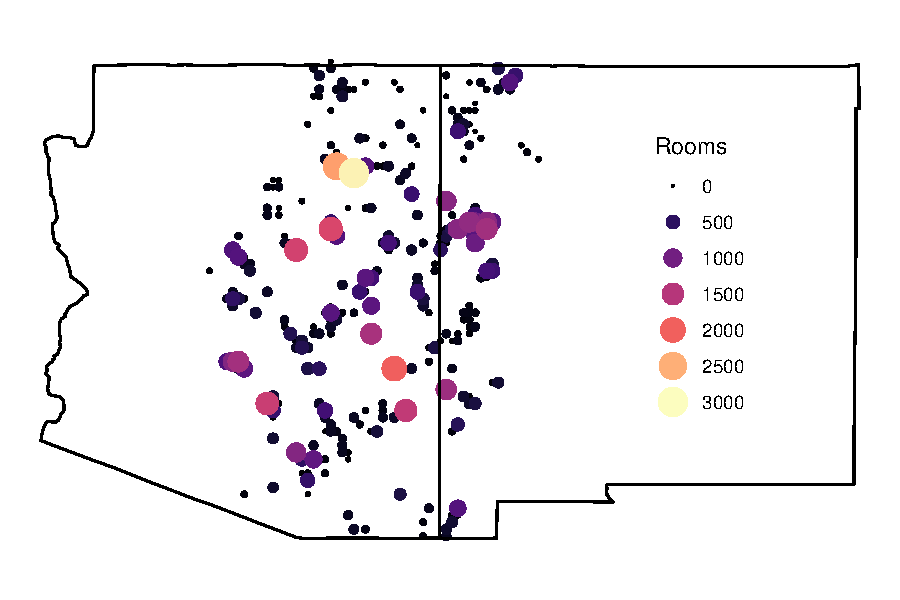
\includegraphics[width=.9\linewidth]{figures/site_distribution.pdf}
\caption{The \emph{Southwest Social Networks} dataset, version 1. (TODO more detail and include network figures here?)} 
%Each line connects a pair of archaeological sites. Line color corresponds to the similarity of the artifact distributions between the pair. A similarity coefficient of 1 means that the sites share the exact same decorated ceramic wares in the exact same proportions, and a coefficient of 0 means there is no overlap in the ceramic assemblages. This similarity network can be interpreted as the degree of social interaction and cultural transmission between sites, whether via migration, trade, or copying. Networks are shown over successive 50 year time spans, starting at 1200 CE. A relatively stable network configuration starting at 1200 CE is interrupted by climatically-forced migrations near the end of the 1250 time step.}
\label{fig:network-plot}
\end{figure}

\subsection*{Least-Cost Networks}
Distance ultimately constrains social interaction, as the further one travels to interact with a partner the greater will be the cost in time, money, and energy. Distance makes it more difficult for face-to-face interactions, which in turn makes it difficult to monitor conditions in potential migration destinations \parencite{Anderies2011a}, the resources and reputation of potential interaction partners \parencite{Fafchamps2007}, and increases the metabolic costs of transport \parencite{Drennan1984}. Modelling spatial structure in the SWSN data is necessary to control for spatial dependence in statistical analyses of these data. To accomplish this, I calculate the least-cost network between all sites in the SWSN network. The topography of the study area was represented using 90m SRTM DEM, resampled to 250m to reduce computation time and reduce fine-scale topographic noise. A cost matrix was calculated containing, for each DEM cell, the amount of time in seconds it would take a foot traveler to move to each of the 16 neighboring cells. Time costs were calculated using a version of Tobler's hiking function, which estimates walking speed from terrain slope. The function was modified to make it isotropic (i.e. averaging the uphill and downhill walking speeds) and adding an extra penalty to very steep slopes consistent with human cognitive biases \parencite{Pingel2010}. This cost matrix (time) was then inverted to represent conductance (speed), facilitating a sparse matrix representation and estimation of least cost paths using efficient graph theoretic algorithms \parencite{Etten2014}. The resulting transition matrix was used to calculate all pairwise isotropic least cost paths between the centroids of each pair of 10km grid cells containing archaeological materials. 

\subsection*{Spatial Interaction Models}
Spatial interaction models are used across the social and natural sciences \parencite{Wilson1971,Fotheringham1989,Sen1995,Bavaud2008,Murphy2010,Head2015}. In a regression context, a spatial interaction model estimates the pairwise flow -- resources, migrants, information -- among entities as a multiplicative function of predictor influencing the production and attraction of flows as well as measures of their mutual separation or other generalized costs of moving. Archaeologists have used \textit{statistical} spatial interaction models sparingly \parencite{Tobler1971,Hodder1974,Johnson1990ChumashAnalysis} because of the rarity of archaeological data on social interaction strength, although the method is common in simulation studies where data quality is less of a restriction \parencite{Bevan2013, Evans2011, Davies2014,Paliou2016}. The conceptual justification for the use of spatial interaction models on archaeological networks is similar to that used in molecular ecology \parencite{Murphy2010}, with information flows among a spatially-structured metapopulation measured by the divergence of those populations \parencite{Mesoudi2018}. Data of this type have three features that make traditional statistical spatial interaction modeling difficult. These are: 1) the data are bounded between 0 and 1, 2) the measures are pairwise symmetric 3) we have no exact functional expectations for the specific terms in the spatial interaction model because empirical work on this scale and type is rare. To address these issues, I used generalized additive models \parencite{Wood2006a}, a semiparametric extension to generalized linear models useful for estimating more complex interaction models \parencite{Lebacher2018}.

Specifically, I fit models of the form

\begin{equation}
    logit\left(D_{ijt}\right) = f(dist_{ij}) + f_t(EOF_{ij}) + \tau_{it} + \tau_{jt} + \epsilon_{ijt}
\end{equation}
where the logit function maps the data from $[0, 1]$ to $[-\infty, +\infty]$, $t$ is the time step, $f()$ is an arbitrary function estimated during model fitting using penalized cubic regression splines, $\tau_i$ and $\tau_j$ are time-varying random effects for the nodes incident on each edge, and $\epsilon$ is Gaussian error. This model assumes only that information flows are at equilibrium with settlement population, not that the populations themselves are at equilibrium \parencite{Wilson2008}. The $\tau$ terms account for the non-independence of edges that share a node, and were estimated using a maximum likelihood population effects correlation structure appropriate for pairwise data \parencite{Clarke2002}. I compared the AIC, BIC, and $R^2$ of models fit using maximum likelihood with and without the EOF terms, and refit the best performing model using restricted maximum likelihood \parencite{Clarke2002,Shirk2018}. 

\section*{Results}

\subsection*{Six drought patterns explain 83\% of observed drought variability in the American Southwest}
The leading 6 PC time series together explain 83\% of the SPEI variance from the 100 year observational record (Figure \ref{fig:scree}). The principal components (PCs) represent SPEI time series that are maximally representative of the entire data set (Figure \ref{fig:pc-obs}). I rotated the 6 PCs before mapping, in order to capture more physically meaningful patterns and minimize statistical artifacts. PCs beyond the leading 6 were not retained for rotation and mapping, as they represent spatially and temporally incoherent variability and spurious correlations introduced by sampling error in the observational record. 
%todo explain here why exactly cut off at 6 and not 5 or 7

\begin{figure}[!ht]
\centering
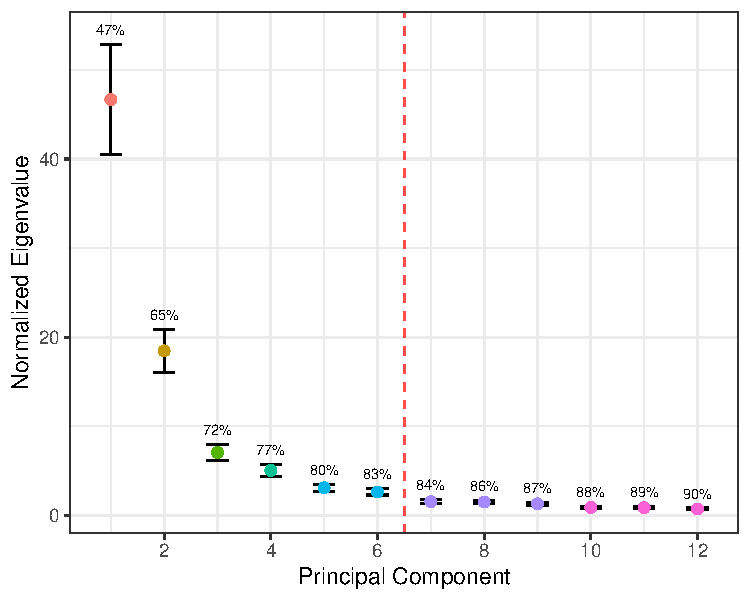
\includegraphics[width=.8\linewidth]{figures/scree.pdf}
\caption{Leading 12 principle components, in order of decreasing eigenvalues, along with the cumulative percent of the variance explained by the leading PCs. Standard errors calculated using North et al.'s rule of thumb \parencite{North1982}. PC's with the same colors (5-6, 7-9, 10-12) are degenerate multiplets, meaning they cannot be clearly distinguished from one another given the sampling variability in the observational dataset. The dashed line represents the truncation point, beyond which PCs were not retained for further analysis. The leading 6 PCs collectively explain 83\% of drought variability in the observed drought record.}
\label{fig:scree}
\end{figure}

\begin{figure*}[!ht]
\centering
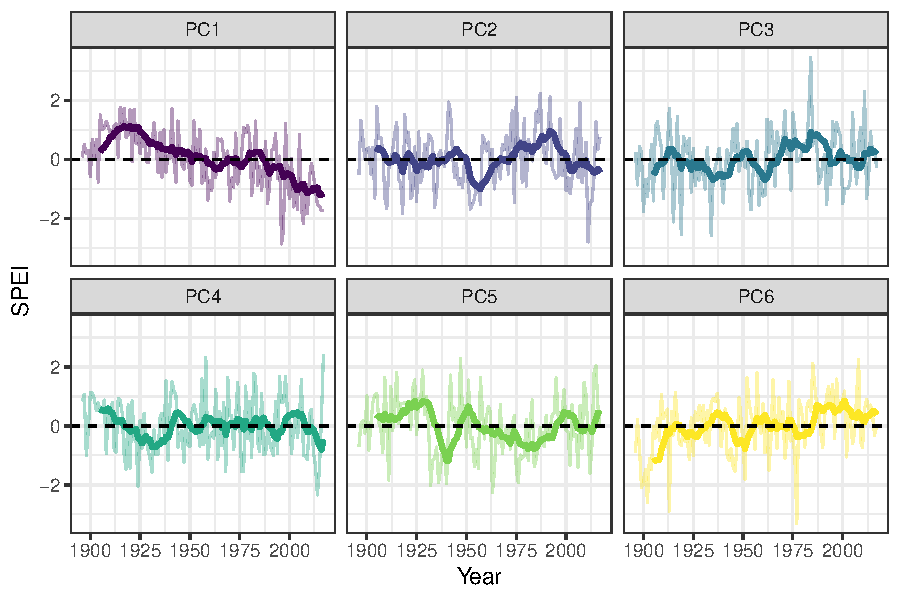
\includegraphics[width=.7\linewidth]{figures/pc_obs.pdf}
\caption{Time series associated with the leading 6 PCs for the observational period, after varimax rotation. SPEI values can be interpreted as z-scores in a normal distribution (i.e. a value of 1 is one standard deviation wetter than average for that location, -1 is one standard deviation drier). The dashed line corresponds to a SPEI value of 0 (i.e. average climatic water balance). 10 year moving averages superimposed over raw annual values. Observed PC time series are shown here to aid in interpretation of the underlying physical mechanisms, and all save PC6 are present in an independent SPEI reconstruction from the last millennium.}
\label{fig:pc-obs}
\end{figure*}

\subsection*{Different drought patterns are associated with different zones of oceanic or continental influence}
To reveal the latent spatial structures associated with the temporal modes of variability, I mapped the spatial patterns associated with each of the leading 6 PCs (Figure \ref{fig:eofs}). The results are robust, recurring patterns of spatially-coherent variability, and can be interpreted as the degree to which 100 year record at each grid cell correlates with the associated rotated PC time series. These spatial patterns are known as the (rotated) empirical orthogonal functions (EOFs). The patterns are consistent regardless of the exact SPEI time scale used to calculate them, which supports their robustness. The spatial and temporal patterns associated with the leading 6 PCs allows us to trace the sources of each mode of variability back to the global climate system.

\begin{figure*}[htbp!]
\centering
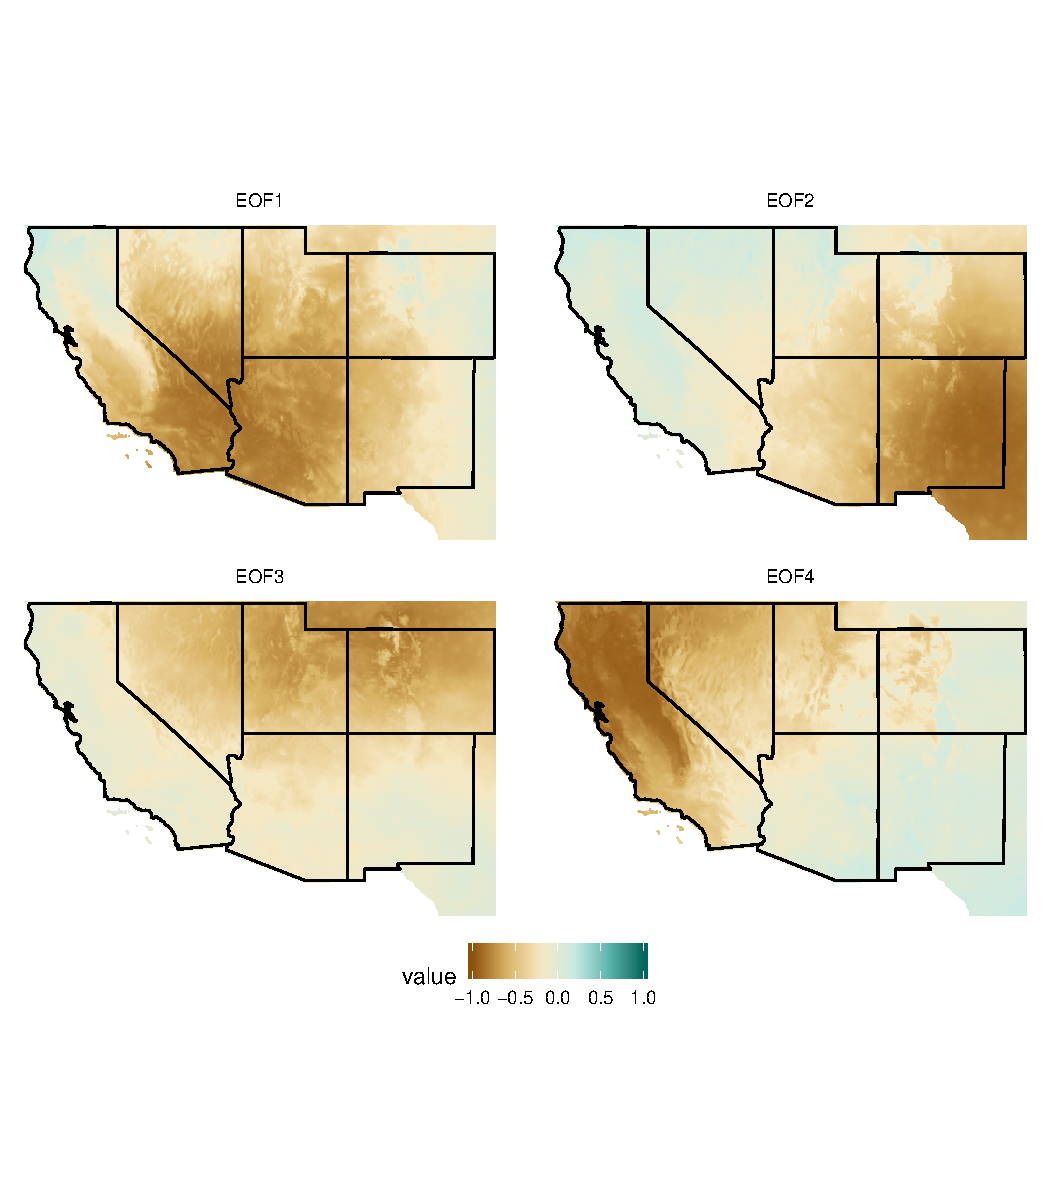
\includegraphics[width=.8\linewidth]{figures/reof_observed.pdf}
\caption{Leading 6 rotated empirical orthogonal functions (EOFs). The empirical orthogonal functions are the spatial patterns associated with their respective principal component time series in Figure \ref{fig:pc-obs}. The EOFs are the eigenvectors of the space-time covariance matrix, and the PCs are the eigenvalues. The leading six EOFs, which together explain 77\% of interannual drought variability in the observational record, were then subjected to varimax rotation, to make the spatial patterns more physically meaningful by relaxing the spatial orthogonality constraint.}
\label{fig:eofs}
\end{figure*}

I determined the origins of each drought pattern by examining the EOF maps, along with the correlations of the PCs to global sea surface temperature and examining extreme dry and wet periods in each observed PC. EOF1 reflects southwesterly flow from the tropical pacific, bringing moisture across the low desert zones of California and Arizona. The pattern attenuates with gains in elevation, as distance from the ocean increases. PC1 shows an broad drying trend to the present day, possibly related increased evaporative demand due to recent warming. EOF2 similarly represents southeasterly flow from the Gulf of Mexico, centered eastern New Mexico. As with EOF1, the pattern attenuates with increasing elevation and distance from the ocean due to orography and continentality, respectively. It represents cyclonic storms coming from the Gulf of Mexico, in turn influenced by variability in Atlantic sea surface temperatures. PC2 shows a major dry period centered on the Texas/New Mexico drought of 1956. EOF3 represents northerly flow associated with polar continental cold fronts, and its associated PC shows a wet peak in the 1983 Salt Lake City floods. EOF4 represents the influence of westerly flow off the Pacific Ocean and the orographic effect of the Sierra Nevada mountains intercepting this flow, and is associated with coastal droughts in California such as the Dust Bowl and 1924 drought. EOF5 is centered over the great plains and attenuates across the Rocky Mountains, and was most strongly expressed during the Dust Bowl of the 1920s. EOF6 is centered on the the Colorado Plateau, likely reflecting hot continental air masses, and is the only pattern not also visible in coarse-resolution reconstructions.

%The mode of variability here is likely temperature dependent, reflecting interactions with radiation at increased elevation.  Variability here is likely linked to Atlantic multidecadal variability. Perhaps the 4 corners high. Arctic oscillation and North Atlantic oscillation for EOF 6. Yes, EOF6 is the AO/NAO, associated with cold dry winters in the west during its positive phase. Consistent with sst correlations and timing of extreme events (1977). (Myoung et al 2015). PC6 shows up with the 1977 drought in Colorado and California. (TODO) mention sst correlations here too. (TODO fix)

%\begin{figure}[!ht]
%\centering
%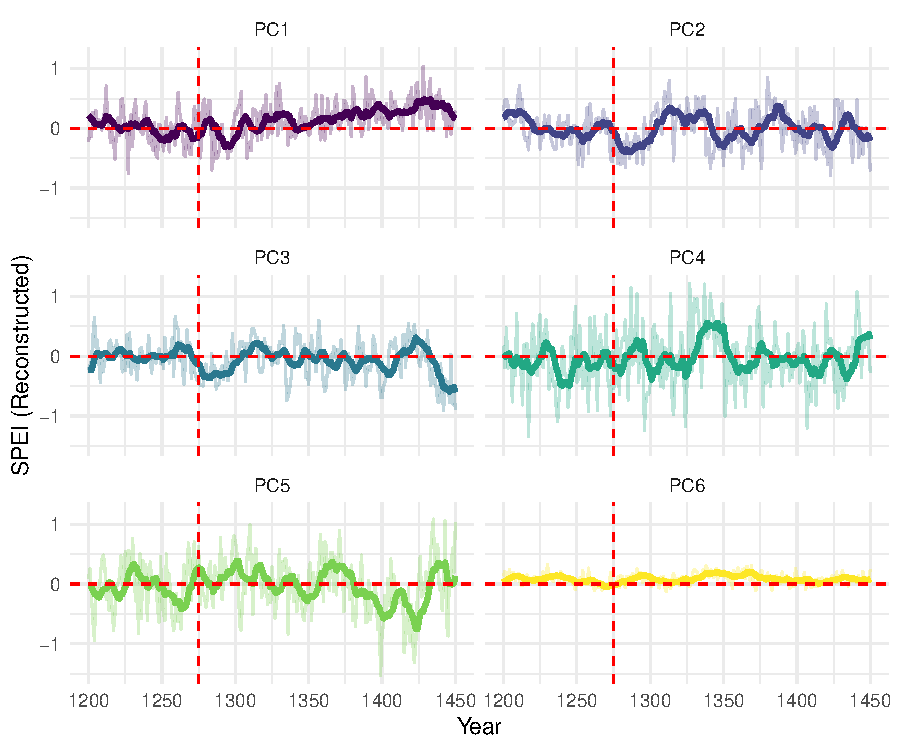
\includegraphics[width=\linewidth]{figures/spei_reconstruction.pdf}
%\caption{}
%\label{fig:spei-reconstruction}
%\end{figure}

\subsection*{Hydroclimate variability explains a moderate but clear proportion of the intensity of social interaction}
The null model for our statistical network analysis was that distance alone explains the intensity of social interaction. This null hypothesis was sufficient to explain nearly 35\% of the variance in archaeological dataset. The distance-only model fitted with the exponential deterrence function predicts a rather sharp falloff in interaction at distance (Figure \ref{fig:distance}). As expected, the resulting distance-based network predicts many strong interactions at close distances. This is confirmed by the residuals of the model, which show long distance transitive ties.

\begin{figure}[!htbp]
\centering
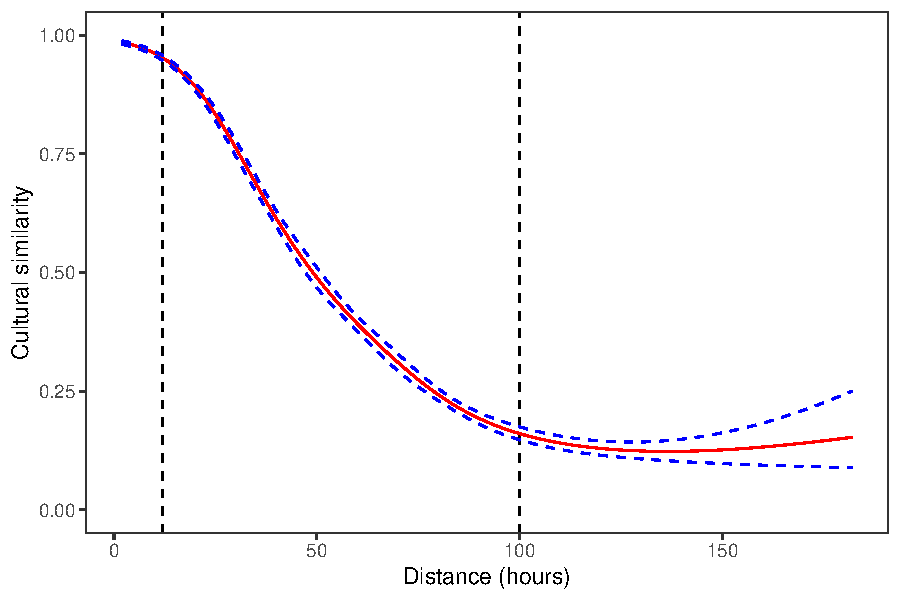
\includegraphics[width=.6\linewidth]{figures/distance_function.pdf}
\caption{Empirical distance deterrence function estimated with a generalized additive model, describing how the intensity of social interaction measured between two settlements decreases as a function of their distance.  (TODO fix axis labels)}
\label{fig:distance}
\end{figure}

A model predicting cultural similarity using distance and climatic dissimilarity, measured as the absolute difference between the EOF loadings of a pair of sites, explains approximately 41\% of the variance in the ceramic similarity data. The increase over the distance-only null model is moderate but statistically significant, and the EOF model is superior in all measures of parsimony and goodness-of-fit. The smooth functions estimated in the EOF model are all close to piecewise linear on the scale of the linear predictor, but the intensity of these functional relationships varies smoothly over time and across EOFs (Figure \ref{fig:smooths}). Increasing distance along a particular EOF sometimes increases the intensity of social interaction, as was expected ahead of time, but some EOFs appear to inhibit social interaction. The smoothness penalty also selects some EOFs out of the model entirely by estimating functions close to a flat line, and almost all the functions are flat when the climate differences are less than 0.2. Surprisingly, the fluctuations in the effect size of a particular EOF have no clear association with the sign of the associated PC amplitude time series reconstructed for each period, suggesting that additional dynamic processes are in effect on time scales longer than a single generation. 
%todo explain what this means for people

%todo cite hill eta l 2015 for changing in the relative explanatory power of distance and eofs before and after the period of drought and social disruption

\begin{figure*}[!htbp]
\centering
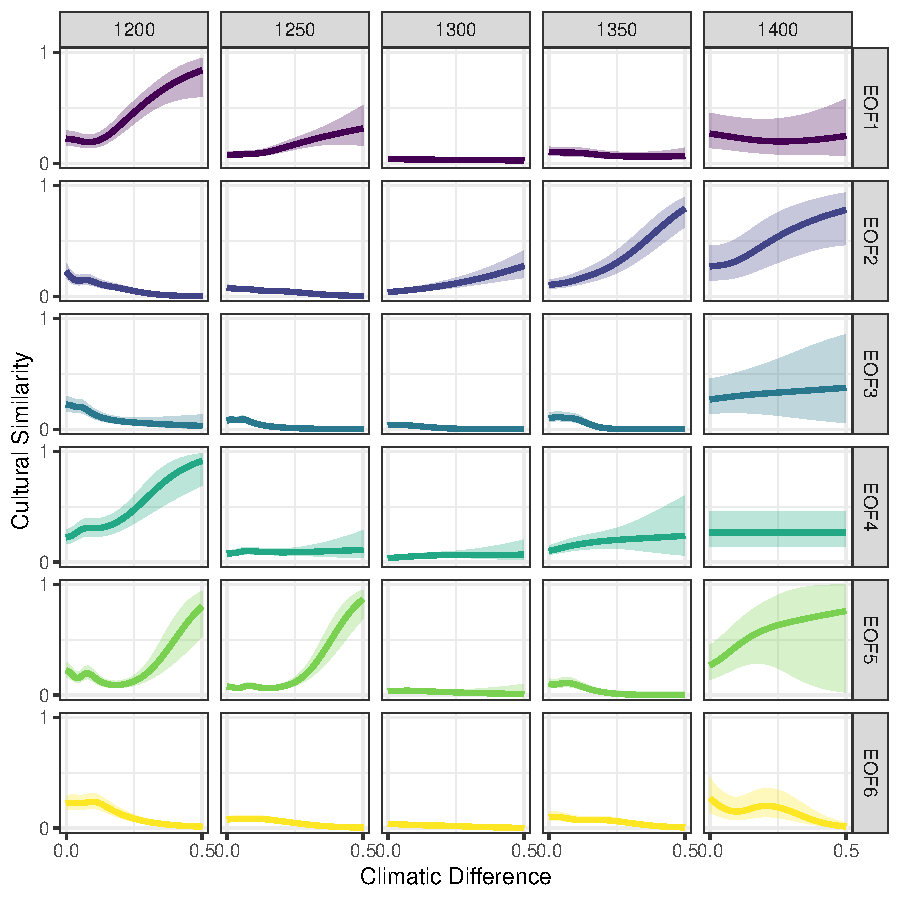
\includegraphics[width=.8\linewidth]{figures/smooths.pdf}
\caption{Estimated smooth functions describing how the intensity of social interaction increases or decreases with increasing distance along each of six spatial drought patterns, compared over five time steps. (TODO explain when eofs inhibit social interaction) Shaded regions correspond to the 95\% confidence intervals for the smooth functions.}
\label{fig:smooths}
\end{figure*}

\section*{Discussion and Conclusions}

The six spatial patterns of hydroclimate variability isolated here are consistent with the general mechanistic understanding of hydroclimate variability in the American Southwest. These patterns represent different zones of moisture transport, reflecting the influence of topography and marine or continental moisture sources \parencite{Liu2010, Hu2011}. These spatial and temporal drought patterns, and their hypothesized forcings from the global climate system, are largely consistent with those from other studies using varied observational data and time windows \parencite{Comrie1999,Cook1999,McCabe1999,McCabe2004,Ryu2010,Seager2014,Herrmann2016}. These same patterns from the observational period also show up in drought reconstructions spanning the past millennium, emphasizing the fact that these are robust, time invariant spatial modes.

%(TODO add citations to mccabe 2004)
Objective measures of hydroclimate variability, rather than point-to-point sample correlations, allow us to isolate the most important drivers of that variability. Droughts and pluvials associated with tropical Pacific and Atlantic influences seem to have been most important for structuring social interaction, with ties connecting these regions greater than expected by chance and distance. Tropical Pacific sea surface temperatures are known to be the primary driver of variability in Southwest, with additional influences from moisture sources in the North Pacific and Atlantic \parencite{McCabe2004}. A disruption in these patterns is thought to be one reason why droughts in this period led to such social transformation, as the networks of social infrastructure that had developed over previous centuries were unable to adapt fast enough to unusual conditions \parencite{Cordell2007}. 

Populations in the late pre-Hispanic Southwest were clearly out of equilibrium \parencite{Hill2004}. Exchange networks take time to develop and effort to maintain. Social dynamics such as free-riding can lead to the breakdown in this critical social infrastructure when it is most needed \parencite{Kohler1996}. Yet the change of the functional forms for the EOF patterns over time still points to dynamics occurring longer than our 50 year time scales. Future studies should leverage these findings in the construction of dynamic simulation models. It will be important to model the evolution of social flows and physical paths separately \parencite{Bevan2013} in order to capture this time lag effect. This will capture year-to-year variability, as well as the time averaging and bias introduced by the use of archaeological similarity data to represent dynamic social processes \parencite{Crema2014}. 
%todo cite turchin secular cycles for possible waxing and waining of social infrastructure


%EOF 1 is strongly positive flooding increasing after 1350, corresponding to flooding in the hohokam region, period of high variability in EOF2. Also corresponds to the Salado phenomenon.

In spite of the robustness of these spatial patterns, there remains considerable diversity in the functional responses of human social networks to these drought patterns. Differences in drought regime are just as likely to inhibit social interaction as they are to enhance it. One possible explanation is that large-scale climate regimes also influence the formation of ethnolinguistic groups. Kinship, or perceived kinship (ethnicity) are important for structuring social exchanges \parencite{Nolin2010}. Small-scale, quotidian interactions may have tracked shared ethnolinguistic affiliation, while interregional exchange may have occurred higher up a sociopolitical hierarchy. The flows of goods and information often proceeded hierarchically, a dynamic poorly-captured in simple spatial interaction models \parencite{Crumley1979}. Perhaps then the strongest flows were between sociopolitical elites at terminal sites.
 
The residuals from the fitted network models retain unexplained structure. These broadly correspond to large cultural clusters, a common feature in social networks that is not accounted for by either distance or drought variability. On a micro scale, the residuals display a pattern of high transitivity and triad closure, which is to say there are a great many more closed triangle structures than would be expected by chance. Although this feature is common in human social networks, it is also to be expected from the semi-metric nature of the data, as full transitivity is to be expected in a metric with subject to the triangle equality. Statistical methods specifically designed for such structures may be preferable in future work \parencite{Stillman2017}. In addition, the archaeological data are not spatially extensive enough to sample the full range of hydroclimate variability. Given the relative spatial scales of our environmental and cultural data, there is a risk that many different correlated climate patterns will be indistinguishable at the scale of the cultural data. Correlation between competing hypotheses as a source of error in model selection using information criteria \parencite{Shirk2018}. In spite of these shortcomings, these results highlight two more novel points: the importance of objective, physically-meaningful measures of drought spatial variability and that social interaction dynamics are out of equilibrium with the biophysical environment. 

%risks not efficiently pooled \parencite{Fafchamps2007}, dynamics are a reason
These results have utility beyond the prehistoric North American Southwest. They are key for understanding the geography of human adaptation to climate and climate change. Prehistoric exchange infrastructure evolved in part in response to robust, time-invariant spatial climate structure. The EOF patterns acted as the selective environment in which norms and institutions regulating social interaction emerge. Social responses adapted to a particular mode of variability can be fragile to changes in that variability \parencite{Janssen2007}. (TODO expand here if space allows?). These findings emphasize the importance of institutional evolution in the developing world, that increases the robustness of human populations to environmental variability.


%These patterns have been discussed in the context of a ``bi-modal precipitation distribution'', distinguishing between regions with both summer and winter dominant precipitation (PC1) and those with just summer dominant precipitation (PC2). Only growing season (summer) variability is measured here, but this pattern is also consistent with winter moisture variability, as the 24 month SPEI index integrates the long lag effects of winter moisture and the summer and winter patterns are governed by similar atmospheric teleconnections to Pacific SST variability. The strength of the summer monsoon has a strong soil moisture memory effect, and is influenced by the preceding winter's precipitation.

%zuni and hopi



%The evidence for conflict and warfare is equivocal \parencite{Kohler2014, leblanc} but largely points to increased resource variability as a source of conflict. 



%This work says nothing about the role of drought in \textit{producing} similarity, such as a drought leading to many migrants, but rather looks at long term patterns in the costs and benefits of traveling between specific pairs of settlements. This is because I integrate out the mean of each site to get attractiveness, effectively integrating out utility measures \parencite{Bavaud2002,Bavaud2008}. So I am specifically looking at the ``deterrence'' effect of climate distances, that is how climate influences the ``effective distance'' between sites by altering the costs and benefits of interaction.

%There are also different social process at play. Food transfers are thought to have occurred primarily in the context of informal sharing within kin groups, reciprocal exchange at ritual ceremonies and festivals, and residential mobility on the scale of one to three generations \parencite{Hegmon1991,Hegmon1996,Varien1999,Cordell2007,Spiemann1983}.



%But there is evidence for long distance exchange between New Mexico and Great Plains cultures \parencite{Spielmann1983} which would be consistent with that pattern influencing exchange. 




%Exchange often occurs in a ritual context (TODO Plog 19xx, Ford 1972).



\printbibliography

\end{document}


